\documentclass[10pt,oneside,swedish]{lips}
\usepackage{float}

%\usepackage[square]{natbib}\bibliographystyle{plainnat}\setcitestyle{numbers}
%\usepackage[round]{natbib}
\bibliographystyle{IEEEtran}

\title{Användarhandledning}
\author{Projektgrupp 13}
\date{14 december 2022}
\version{1.0}

\reviewed{Hannes Nörager}{2022-12-14}
\approved{}{2022-12-14} %Approved ska vara Anders efter han har gett ett OK att 1.0 kan fastställas.

\begin{document}
\projecttitle{Taxibil-robot}

\groupname{Projektgrupp 13}
\groupemail{TSEA29_2022HT_E7-Grupp13@groups.liu.se}
\groupwww{https://gitlab.liu.se/da-proj/microcomputer-project-laboratory-d/2022/g13}

\coursecode{TSEA29}
\coursename{Konstruktion med mikrodatorer}

\orderer{Anders Nilsson, ISY, Linköpings universitet}
\ordererphone{013-28 26 35}
\ordereremail{anders.p.nilsson@liu.se}

\customer{Anders Nilsson, ISY, Linköpings universitet}
\customerphone{013-28 26 35}
\customeremail{anders.p.nilsson@liu.se}

\courseresponsible{Anders Nilsson, ISY, Linköpings universitetn}
\courseresponsiblephone{013-28 26 35}
\courseresponsibleemail{anders.p.nilsson@liu.se}

\supervisor{Peter Johansson}
\supervisorphone{013-28 1345}
\supervisoremail{peter.a.johansson@liu.se}

\smalllogo{../Figures/LiU_primary_black} % Page header logo, filename
\biglogo{../Figures/logo} % Front page logo, filename

\cfoot{\thepage}
\begin{document}
\maketitle

\cleardoublepage
\makeprojectid

\begin{center}
  \Large Projektdeltagare
\end{center}
\begin{center}
  \begin{tabular}{|l|l|l|l|}
    \hline
    \textbf{Namn} & \textbf{Ansvar} & \textbf{Telefon} & \textbf{E-post}\\
    \hline
    Linus Thorsell & Projektledare & 0765612171 & linth181@student.liu.se\\
    \hline
    Oscar Sandell & Testansvarig & 0709416866 & oscsa604@student.liu.se\\
    \hline
    Hannes Nöranger & Utvecklare & 0733118779 & hanno696@student.liu.se\\
    \hline
    Johan Klasén & Dokumentansvarig & 0730982555 & johkl473@student.liu.se\\
    \hline
    Zackarias Wadströmer & Utvecklare & 0706142029 & zacwa923@student.liu.se\\
    \hline
    Thomas Pilotti Wiger & Konstruktionsansvarig & 0761708593 & thopi836@student.liu.se\\
    \hline
  \end{tabular}
\end{center}


\cleardoublepage
\tableofcontents

\cleardoublepage
\section*{Dokumenthistorik}
\begin{tabular}{p{.06\textwidth}|p{.1\textwidth}|p{.45\textwidth}|p{.13\textwidth}|p{.13\textwidth}} 
  \multicolumn{1}{c}{\bfseries Version} & 
  \multicolumn{1}{|c}{\bfseries Datum} & 
  \multicolumn{1}{|c}{\bfseries Utförda förändringar} & 
  \multicolumn{1}{|c}{\bfseries Utförda av} & 
  \multicolumn{1}{|c}{\bfseries Granskad}\\
  \hline
  \hline
  1.0 & 2022-12-14 & Första versionen & Grupp13 & Johan Klasén   \\
  \hline
\end{tabular}

\cleardoublepage
\pagenumbering{arabic}\cfoot{\thepage}

\section{Inledning}
\subsection{Bakgrundsinformation}
Det här är användarhandledningen för er autonoma taxibil samt mjukvaran för att kontrollera den. 
Den autonoma taxibilen är utvecklad för att kunna navigera sig genom ett vägnät definierat enligt en banspecifikation, se \ref{appendix:banspec}, från en punkt till en annan utan att kollidera med eventuella hinder på vägen. Alternativt styras manuellt med tangentkommandon från en extern dator.

\subsection{Ingående delsystem}
Produkten består av en bil med motorer och servon samt kontrollteknik i form av en kommunikationsmodul, en styrmodul, en sensormodul samt en extern applikation.

\subsection{Beroenden till andra system}
Fordonet är beroende av en extern dator för kontroll via den externa applikationen. Datorn måste köra linux och ha en webbläsare samt Python installerat.

\begin{figure}[htbp]
  \centering
  \includegraphics[width=.8\textwidth]{../Figures/Car_Right.jpg}
  \caption{Bilen sedd från höger.}
  \label{fig:car-right}
\end{figure}

\cleardoublepage
\section{Hårdvara}

\subsection{Strömförsörjning}
Bilen får ström från ett 7.2V batteri som ansluts via den/rödsvarta kontakten på bilens vänstra sida, se Figur \ref{fig:car-left}. Batteriet ger ström till sensor- och styrmodulen genom en regnbågsfärgad 10-polig kabel på framsidan av bilen som ansluts till den stående kontakten på bilens ovansida, och till kommunikationsmodulen via en ljusgrå micro-USB kabel i framkant på bilen. Intill kommunikationsmodulen på höger sida av bilen finns en strömbrytare för att stänga av och sätta på bilen, se Figur \ref{fig:car-right}.

\begin{figure}[htbp]
  \centering
  \includegraphics[width=.8\textwidth]{../Figures/Car_Left.jpg}
  \caption{Bilen sedd från vänster.}
  \label{fig:car-left}
\end{figure}

\subsection{Knappar, sensorer och övriga portar}
Bilens ovansida är försedd med två knappar, en svart knapp fungerar som reset för styrmodulen och en grå knapp fungerar som reset för sensormodulen. På bilens ovansida finns även två liggande kontakter för felsökning av systemet, där den blå är för sensormodulen och den svarta för styrmodulen. För kommunikation mellan de olika modulerna måste även två USB- till 6-pin kablar anslutas. Dessa kopplas från valfri av de övre USB portarna på Rasperry Pi till valfri rad på den stående kontakten bak till vänster på kretskortet, med svart kabel mot den svarta markeringen.

\noindent
På bilens framsida finns en ultraljudsensor. Denna ansluts med en 5 till 4-pins kabel till kretskortet där svart kabel mot den svarta markeringen på kretskortet/sensorn. Bilens kamera ansluts till systemet via en bandkabel direkt till den dedikerade kameraporten på Raspberry Pin.

\begin{figure}[htbp]
  \centering
  \includegraphics[width=.8\textwidth]{../Figures/Car_Top.jpg}
  \caption{Bilen sedd från ovan.}
  \label{fig:car-top}
\end{figure}

\cleardoublepage
\section{Mjukvara}
Appen som styr bilen är skriven som en webb-applikation, detta betyder att för att köra denna måste den hostas någonstans.
I denna användarhandledning kommer detta att göras med hjälp av programmet Live-Server.

\begin{figure}[htbp]
  \centering
  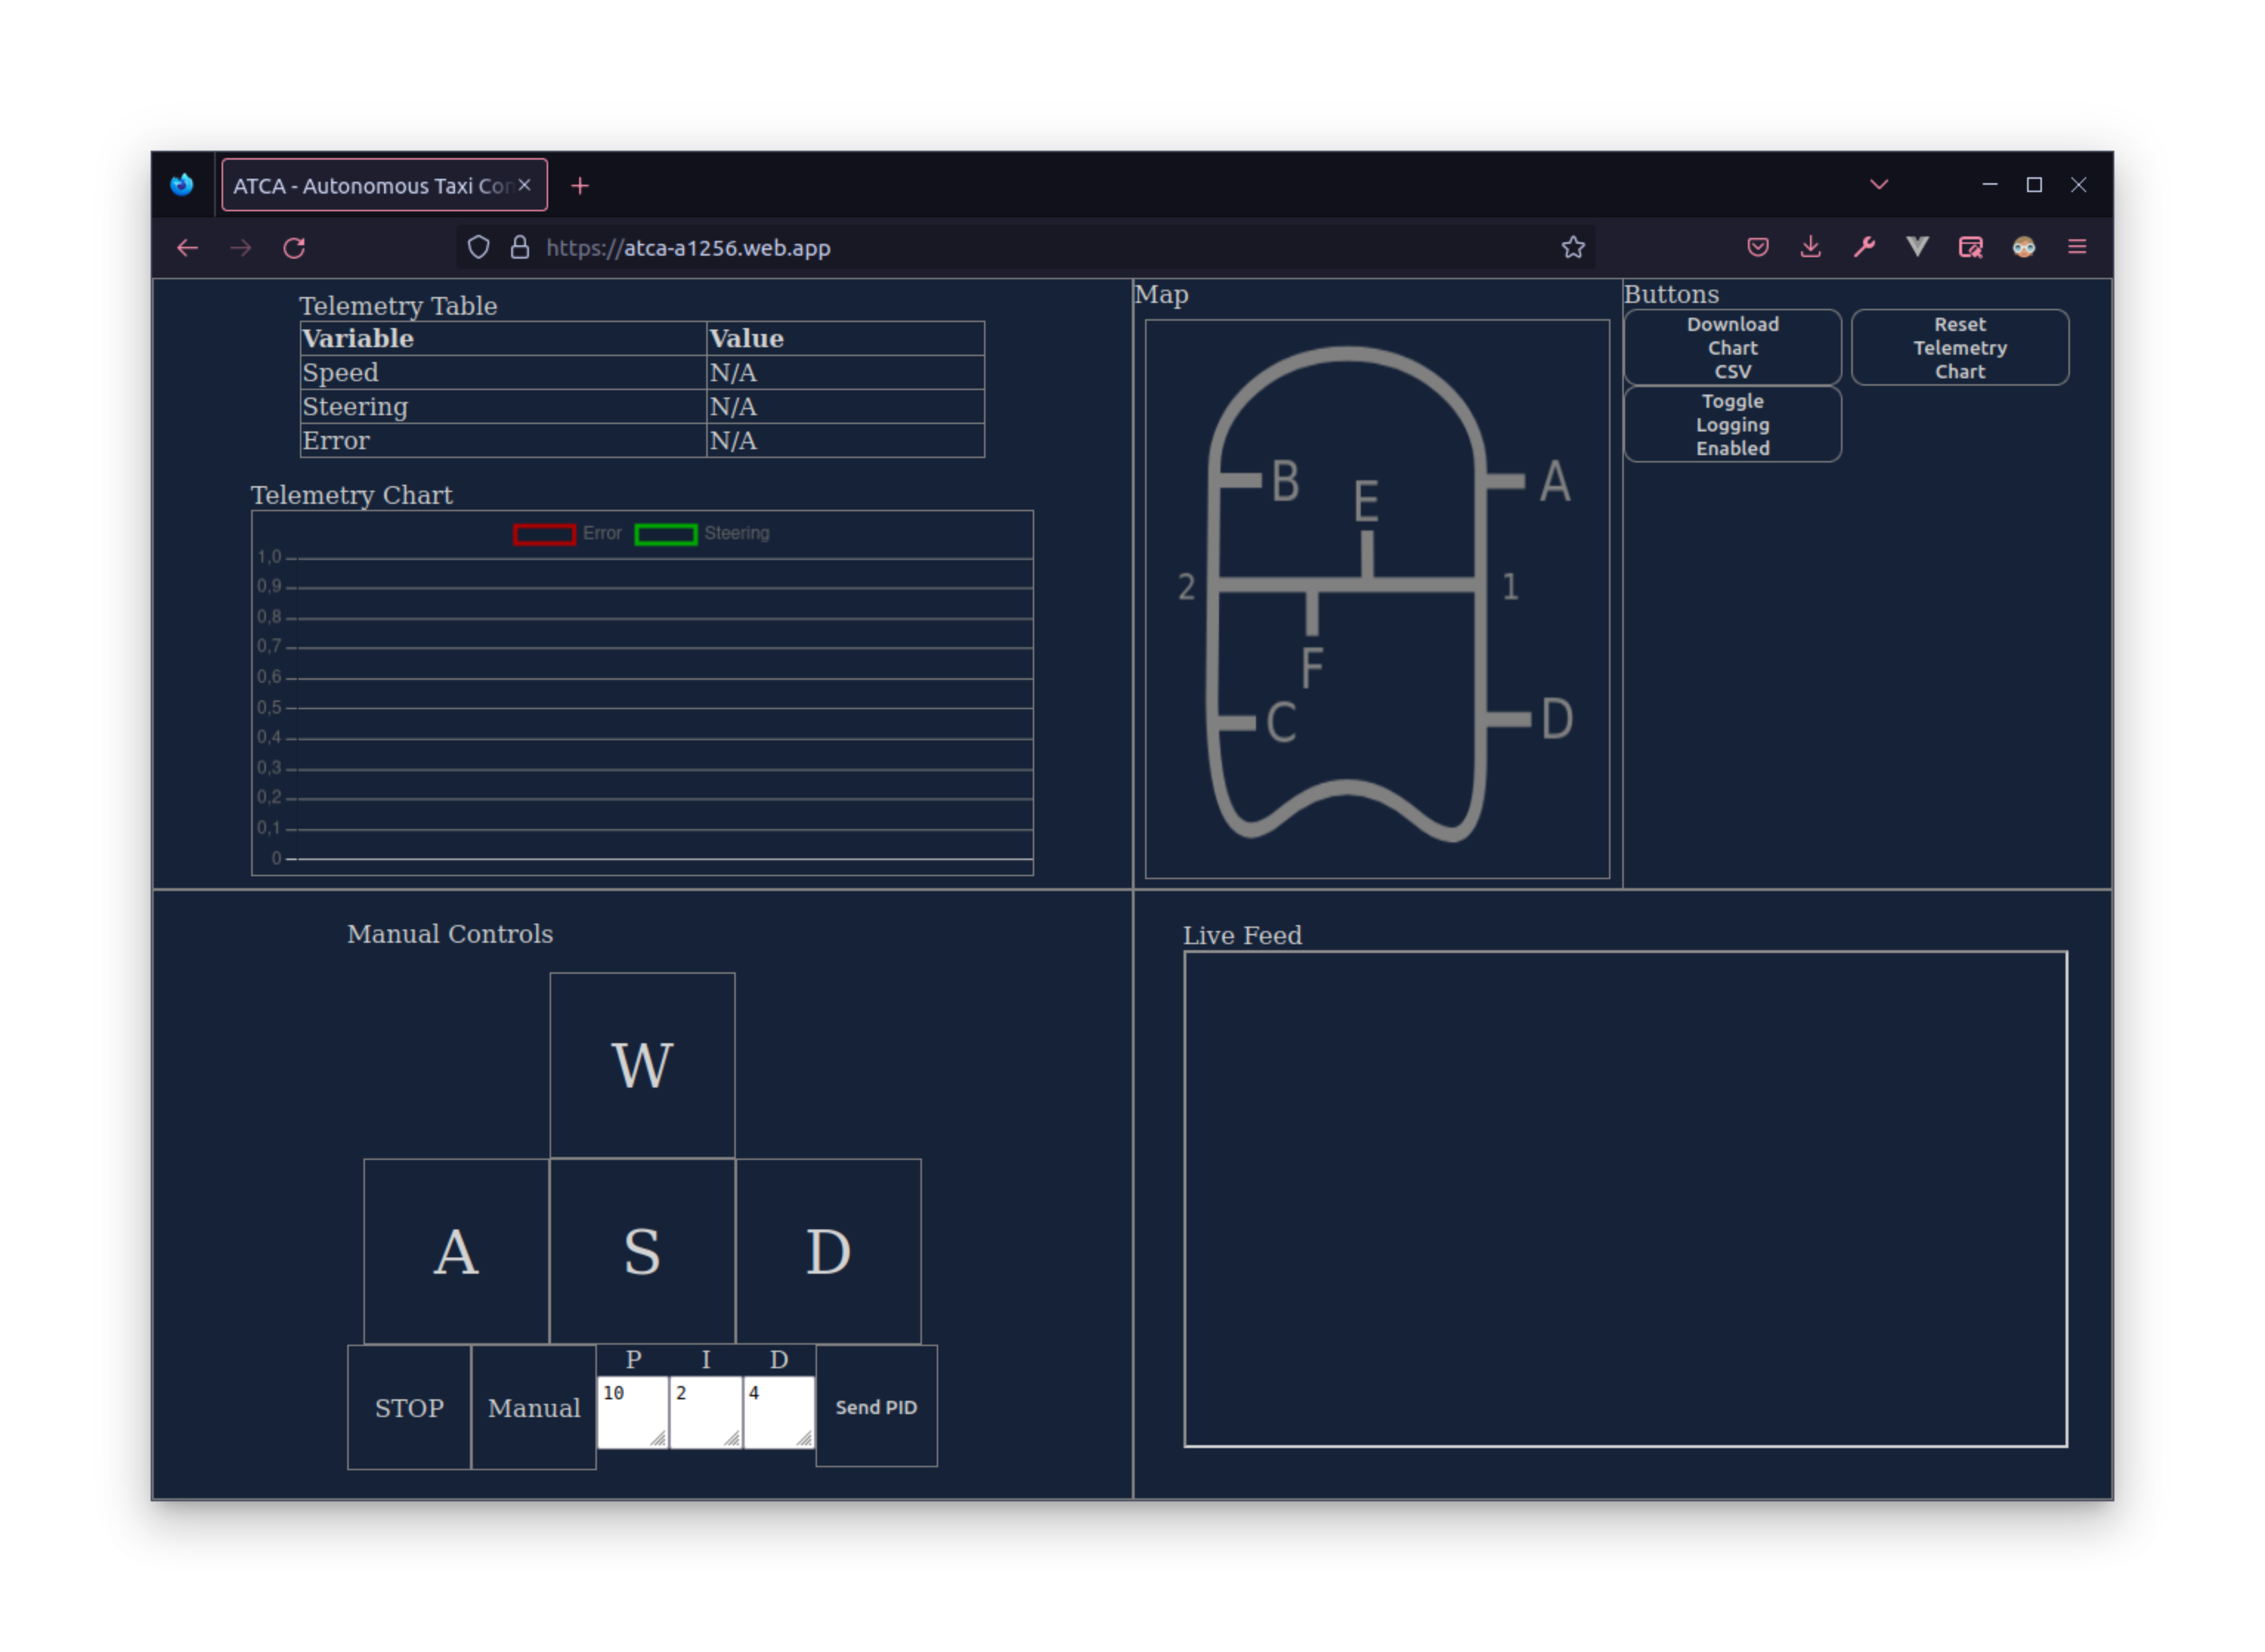
\includegraphics[width=.7\textwidth]{../Figures/app-overview.png}
  \caption{Appens utseende.}
  \label{fig:app-overview}
\end{figure}

\subsection{Installera och kör appen} 

Clona git-repot med följande kommando:
\begin{lstlisting}[language=sh,frame=single, basicstyle=\footnotesize]
git clone https://gitlab.liu.se/da-proj/microcomputer-project-laboratory-d/2022/g13/projekt.git
\end{lstlisting}

\noindent
Navigera till mappen 'app-module'

\noindent
Installera npm och nodejs via följande kommandon:
\begin{lstlisting}[language=sh,frame=single]
sudo apt install nodejs
sudo apt install npm
\end{lstlisting}


\noindent
Installera paketet Live-Server med npm.
\begin{lstlisting}[language=sh,frame=single]
npm install -g live-server
\end{lstlisting}


\noindent
Kör appen med följande kommando:
\begin{lstlisting}[language=sh,frame=single]
live-server
\end{lstlisting}
Nu kommer appen öppnas i din standard-webbläsare.

\cleardoublepage
\subsection{Användande av appen}

\noindent
När appen öppnas kommer den att fråga efter IP addressen av bilen. 
Det är viktigt att både bilen och datorn som skall styra bilen är på samma nätverk.
Se till att bilen är på, ta reda på bilens lokala IP address, skriv in den och starta anslutningen.

\noindent
Nu när appen körs och bilen har anslutits finns det ett par funktioner som går att använda.

\subsubsection{Körande}
När appen startas är bilen i Manual mode och kan då köras med hjälp av W för att åka framåt,
S för att bromsa, A för att svänga vänster och D för att svänga höger. 
För att få bilen att köra autonomt klickar man helt enkelt på knappen under W, A, S, D 
där det står Manual mode, då kommer knappens text ändras till Auto och bilen startar sitt
Autonoma läge.

\subsubsection{Graf / Status}
Tablet som finns högs upp till höger rapporterar senaste telemetriuppdateringen som fåtts från bilen. Grafen som synns under denna loggar  datan och går att styra med hjälp av knapparna högst upp till höger, enligt följande beskrivning:

\noindent \\
\emph{'Download Chart CSV'}: Denna knapp laddar ner all nuvarande grafdata till en .CSV fil som kan öppnas med valfritt kalkylprogram.

\noindent \\
\emph{'Reset Telemetry Chart'}: Denna knapp kastar all nuvarande data i grafen, detta startar helt enkelt om datainsamlingen.

\noindent \\
\emph{'Toggle Logging <Enabled/Disabled>'}: Denna knapp används för att toggla om appen skall logga all telemetri den får, om det står Enabled så sparar den all data och om det står Disabled så ignorerar den all data. Läget Enabled/Disabled ändras genom att trycka på knappen.

\subsubsection{Kartan}
Kartfunktionen är en hel-automatisk graf som visar vart på banan bilen befinner sig i nuläget. Denna uppdateras direkt när bilen befinner sig i autonomt läge och vet vart den är, alltså uppdateras den alltid direkt när den får sitt uppdrag och slutar rapportera när den kört färdigt sitt uppdrag.

\subsubsection{Live feed}
Live-feed funktionen är en live-streamad video från kameran på bilen. Denna fungerar endast när bilen är i Manuella läget då det autonoma läget behöver prioritet för kameran. Men med denna funktion kan man köra bilen utom synlig räckvidd. Så länge bilen är på samma nätverk som applikationen kan denna åka hur långt som helst med låg latens videoöverföring.

\cleardoublepage

\appendix{}
\section{Banspecifikation}
\label{appendix:banspec}
\begin{figure}[H]
    \centering
    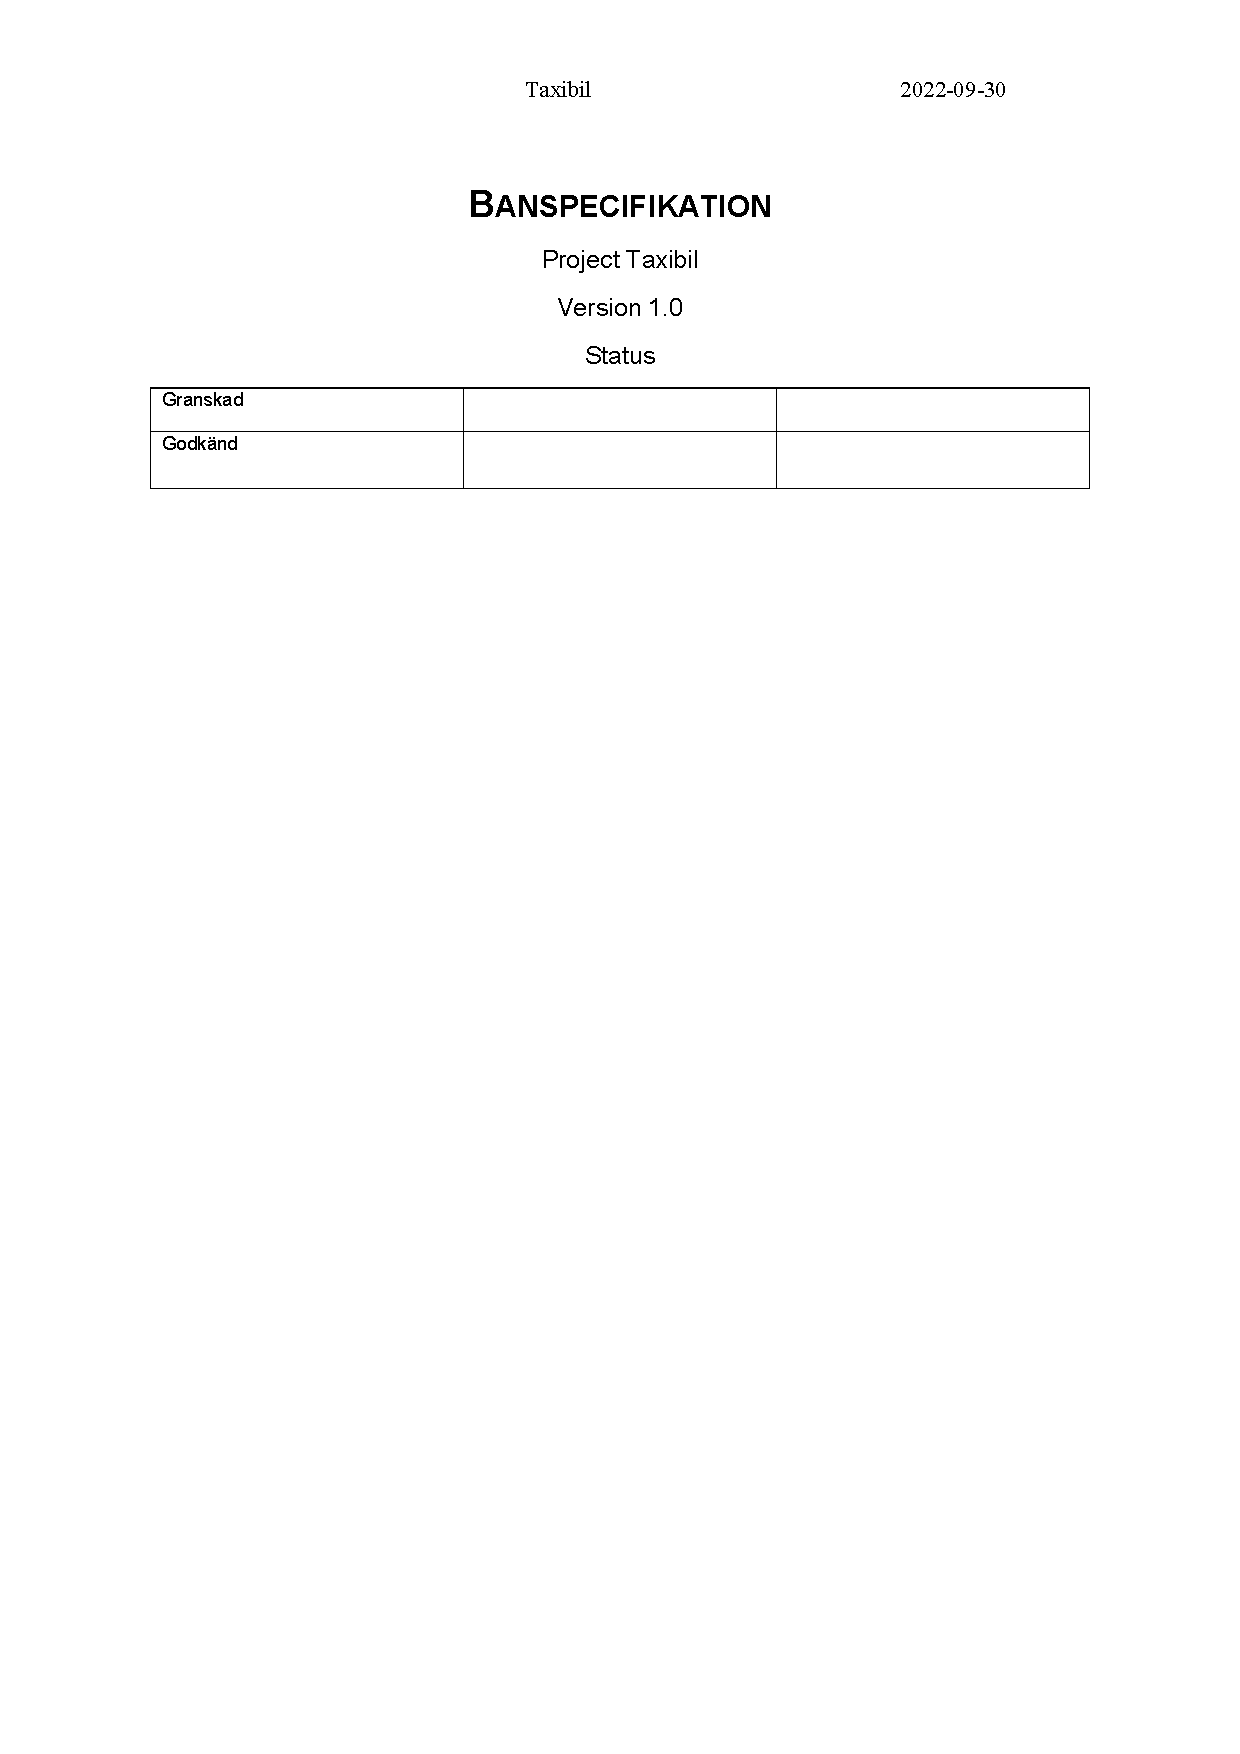
\includegraphics[width=.95\textwidth]{Banspec.pdf}
\end{figure}
\begin{figure}[H]
    \includegraphics[width=.95\textwidth, page=2]{Banspec.pdf}
\end{figure}
\begin{figure}[H]
    \includegraphics[width=.95\textwidth, page=3]{Banspec.pdf}
\end{figure}
\end{document}